\chapter{Study Management}

In this module the \entitytarget{Study} aggregate is used to configure a
study. It defines the valid types of specimens that can be collected, when they
are to be collected from participants, how the collected specimens are
processed, and allows for customization with use of annotations. This aggregate
is made up of the entities and value objects shown in the figure below.

This section first describes the study aggregate and then defines the commands
it handles.

\begin{figure}[h]
  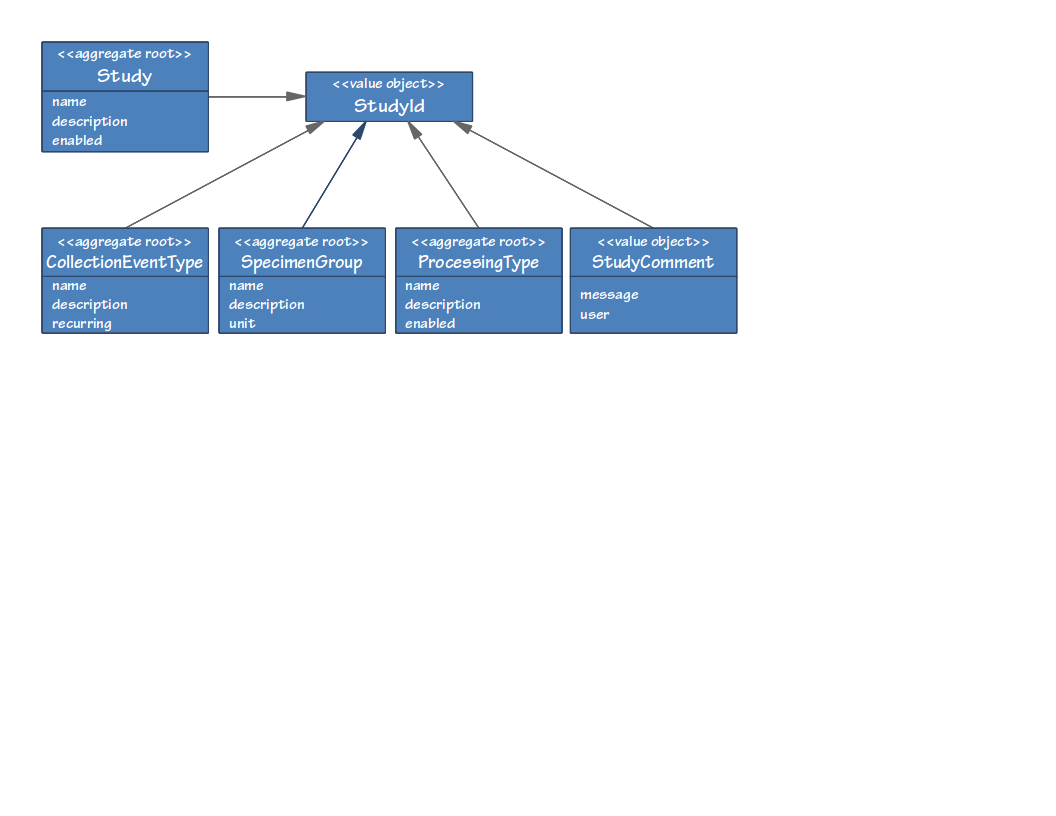
\includegraphics[trim={9mm 85mm 36mm 9mm}, clip,
    width=1\textwidth]{images/study-aggregate}
  \caption{Study aggregate}
  \label{fig:study-aggregate}
\end{figure}

\subsection*{Study}

Represents a collection of participants and specimens collected for a
particular research study. The study name is a short descriptive name that is
usually an acronym used for quick identification. The description contains text
used to give more details on the name and is usually the words that make up the
acronym.

A study can be enabled or disabled. When disabled, changes to its configuration
are possible but patients and specimens cannot be added. When enabled, no
further configuration changes are allowed, and participants and specimens can
be added.

As shown in the Figure \ref{fig:study-aggregate}, the study has collections of
other entitites and value objects which are described below.

\subsection*{SpecimenGroup}

This entity is used to configure a specimen type used by the study.  It
records ownership, summary, storage, and classification information that
applies to an entire group or collection of \entitylink{Specimen}s. A specimen
group is defined either for specimens types collected from participants, or the
types of specimens that are processed.

A specimen group has a name and a description: the name is a short identifying
name that is unique to the study, and the description is optional and can
provide additional details. The unit specifies how the specimen amount is
measured (e.g. volume, weight, length, etc.).

A study can have one or more specimen groups defined.  For specimen collection
to be allowed on a study, at least one specimen group must be defined.

The anatomical source, preservation medium and specimen type are defined using
other value objects discussed in Section \ref{sec:specimen-group}.

\subsection*{CollectionEventType}

A classification name, unique to the \entitylink{Study}, for a visit by study
participants. Each collection event type has one or more specimen groups (see
Section \ref{sec:collection-event-type}).

A study can have one or more collection event types defined. For specimen
collection to be allowed on a study, at least one collection event type must be
defined.

\subsection*{ProcessingType}

Describes a regularly performed specimen processing procedure with a unique
name (unique to the \entitylink{Study}). There should be one or more associated
\entitylink{SpecimenLinkType}s that (1) further define legal procedures and (2)
allow recording of procedures performed on different types of
\entitylink{Specimen}s.

One or more processing types can be defined for a study. For specimen
processing to be allowed on a study, at least one processing type must be
defined.

\subsection*{StudyAnnotationType}

Annotations types allow a study to collect custom named and defined pieces of
data on collection event types (Section \ref{sec:collection-event-type}),
processing events (Section \ref{sec:processing-type}), and participants
(Section \ref{sec:participant-annotations}).

Annotations are optional and are not a requirement for specimen collection or
processing.

\subsection*{StudyComment}

The comment contains a message and the user that added the comment. The date
and time the comment was made is recorded as meta data. A study can have one or
more comments.

\section{SpecimenGroup Details}
\label{sec:specimen-group}

The \entitytarget{SpecimenGroup} entity is composed of the value objects shown
in Figure \ref{fig:specimen-group}.

\begin{figure}[h]
  \centering
  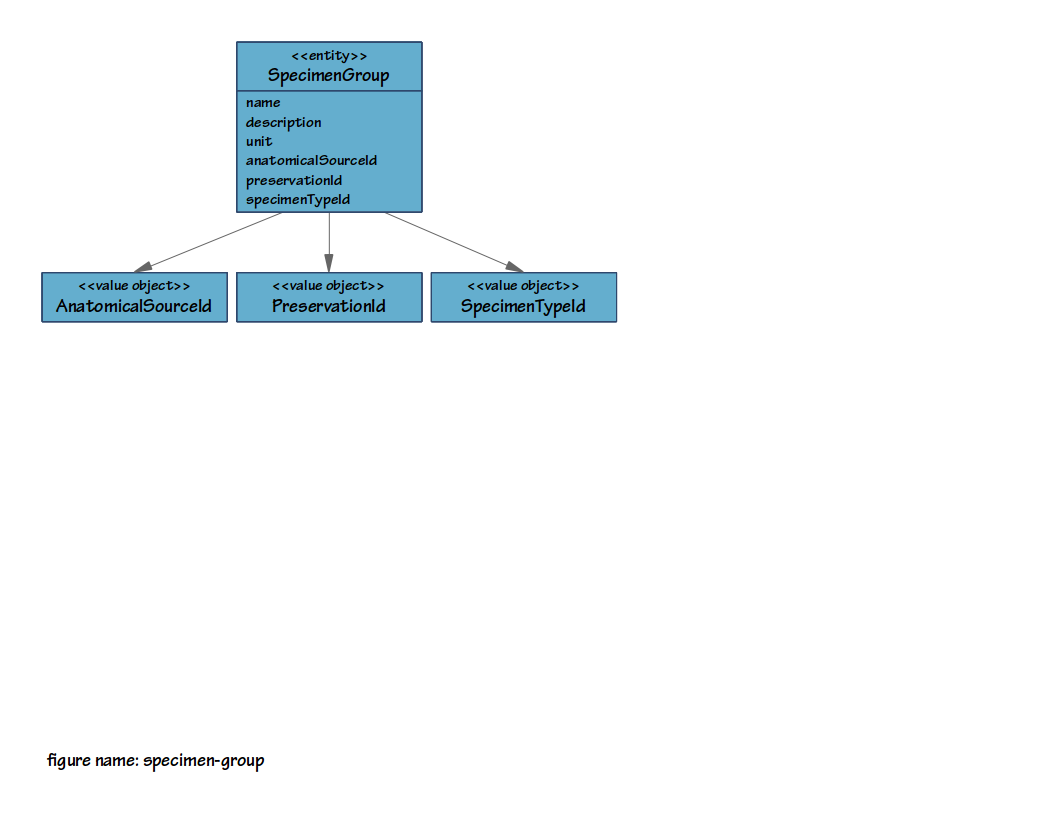
\includegraphics[trim={9mm 162mm 80mm 9mm}, clip,
    width=1\textwidth]{images/specimen-group}
  \caption{SpecimenGroup entity}
  \label{fig:specimen-group}
\end{figure}

\subsection*{AnatomicalSourceId}

An \valobjlink{AnatomicalSource} is a standardized set of regions from a
\entitylink{Participant} \emph{where} a \entitylink{Specimen} is collected
from. Potential examples include: colon, ear, leg, kidney,
etc. \valobjlink{AnatomicalSource} is a value object with a unique ID. They are
defined globally and new ones can be created at any time. They can be accessed
via lookup service described in Section \ref{sec:lookup-service}.

A specimen group contains the ID of a single anatomical source.

\subsection*{PreservationId}

\valobjlink{Preservation} is a value object that describes how a
\entitylink{Specimen} should be preserved/stored by describing temperature
requirements ($^\circ$C), as well as a preservation method (see
\valobjlink{PreservationType}). \valobjlink{Preservation} is also a value
object with a unique ID. They are defined globally and new ones can be created
at any time. They can be accessed via lookup service described in Section
\ref{sec:lookup-service}.

A specimen group contains the ID of a single preservation object.

\subsection*{SpecimenTypeId}

\valobjlink{SpecimenType} is standardized set of classifications that describe
\emph{what} a \entitylink{Specimen} is. Potential examples include: urine,
whole blood, plasma, nail, protein, etc.\valobjlink{SpecimenType} is also a value
object with a unique ID. They are defined globally and new ones can be created
at any time. They can be accessed via lookup service described in Section
\ref{sec:lookup-service}.

A specimen group contains the ID of a single specimen type.

\section{CollectionEventType Details}
\label{sec:collection-event-type}

A collection even type can be configured to collect one or more specimens using
\entitylink{SpecimenGroupCollectionEventType}. Also, it can be configured to
record one or more annotation types using
\entitylink{CollectionEventTypeAnnotationType}. These associations are shown in
Figure \ref{fig:collection-event-type}.

\begin{figure}[H]
  \centering
  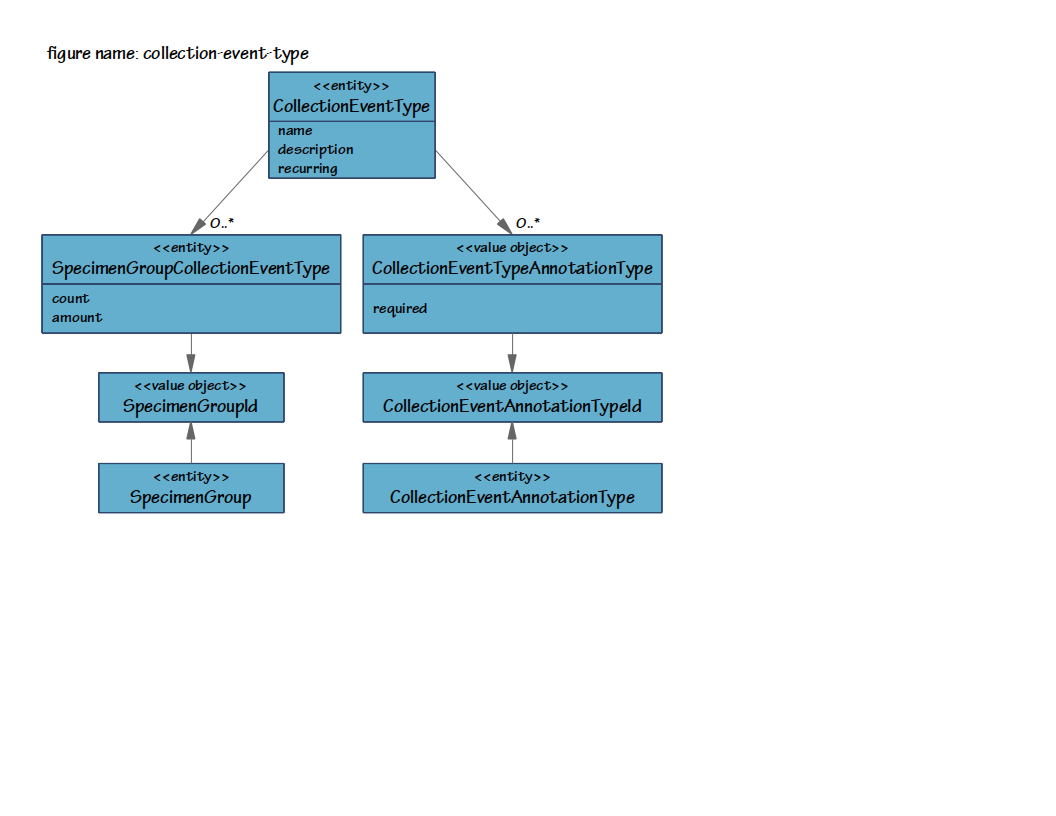
\includegraphics[trim={9mm 70mm 96mm 9mm}, clip,
    width=0.8\textwidth]{images/collection-event-type}
  \caption{Details for the CollectionEventType entity}
  \label{fig:collection-event-type}
\end{figure}

A single specimen group can be used in multiple collection event
types. Also, a single collection event annotation type can be used in multiple
collection event types.

\subsection*{SpecimenGroupCollectionEventType}

\valobjtarget{SpecimenGroupCollectionEventType}s are used to
define which types of specimens (i.e. which \valobjlink{SpecimenGroup}s) need
to be collected with a type of collection event.

The \texttt{count} specifies how many specimens are to be collected. The
\texttt{amount} is the amount of substance that is expected in each collected
specimen, or null if there is no default amount.

\subsection*{CollectionEventAnnotationType}

Collection event annotations are defined using
\valobjtarget{CollectionEventAnnotationType}. One or more of these can be
defined for the study.

\section{ProcessingType Details}
\label{sec:processing-type}

A processing type can be configured to process one or more collected specimens
using \valobjlink{SpecimenLinkType}. Individual specimen link types within the
processing type can also be configured to record one or more annotation using
\valobjlink{SpecimenLinkTypeAnnotationType}. Figure \ref{fig:processing-type}
provides more details for the processing type entity.

\begin{figure}[H]
  \centering
  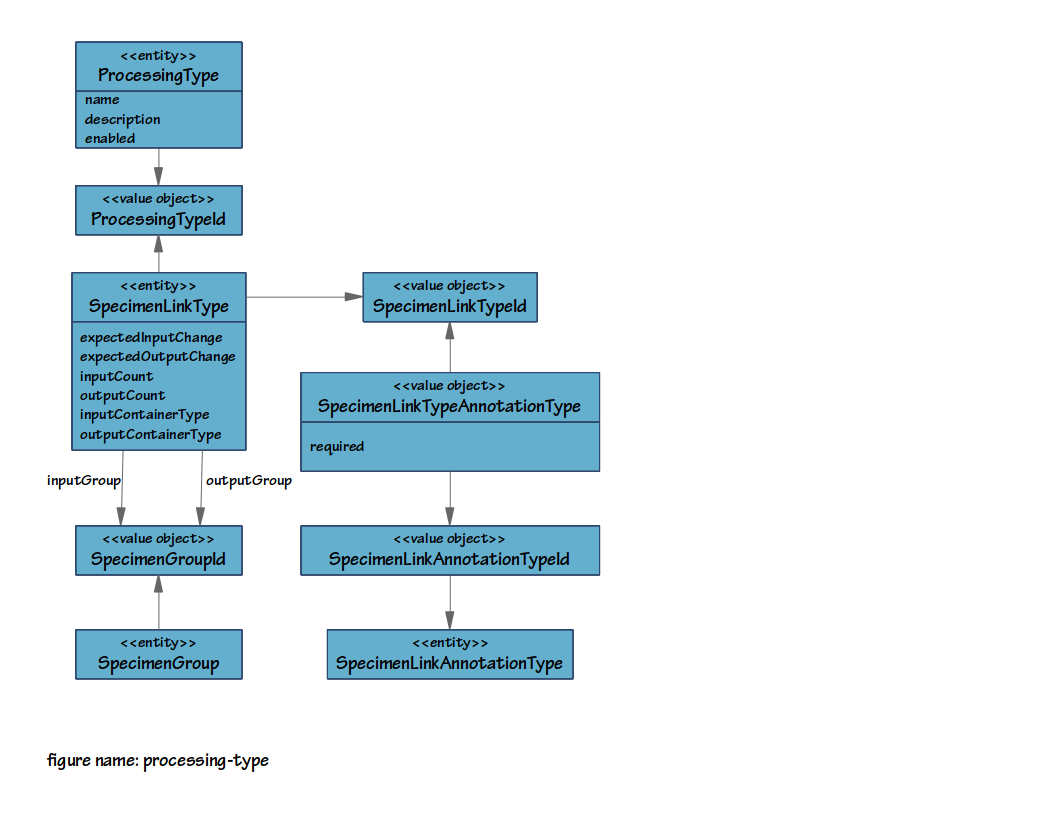
\includegraphics[trim={9mm 48mm 120mm 9mm}, clip,
    width=0.7\textwidth]{images/processing-type}
  \caption{Details for the ProcessingType entity.}
  \label{fig:processing-type}
\end{figure}

Processing of specimens is not allowed until a valid processing type is defined
for the study.

\subsection*{SpecimenLinkType}

 \valobjtarget{SpecimenLinkType}s are assigned to
a processing type, and used to represent a regularly performed processing
procedure involving two \entitylink{Specimen}s: an input, which must be in a
specific \valobjlink{SpecimenGroup}, and an output, which must be in a specific
\valobjlink{SpecimenGroup}.

The \texttt{expectedInputChange} is the expected amount (decimal value) to be
removed from each input. The \texttt{expectedOutputChange} is the expected
amount to be added to each output. The expected input and output change values
can be zero.  The counts in \texttt{inputCount} and \texttt{outputCount} are
the number of expected and resulting specimens, respectively, when the
processing is carried out. A value of zero for output count implies that the
count is the same as the input count. The specimen container type that holds
the input specimens is given in \texttt{inputContainerType}. The specimen
container type that the output specimens are stored into is given in
\texttt{outputContainerType}. If specifying the container types is not required
for one or both of these fields they can be assigned the \texttt{null} value.

To avoid redundancy, a specimen link type may exist only once for a given input
and output specimen group.

\subsection*{SpecimenLinkTypeAnnotationType}

A \valobjtarget{SpecimenLinkTypeAnnotationType} is used to tie a specimen
link annotation type to a specimenlink type. When \texttt{required} is set to
\texttt{true} the annotation value is not allowed to be empty.

\section{Participant Annotations}
\label{sec:participant-annotations}

Figure \ref{fig:study-annotations} show the possible annotations types that can
be configured for a study. Annotations types must be defined before they can be
assigned to the respective entity.

\begin{figure}[H]
  \centering
  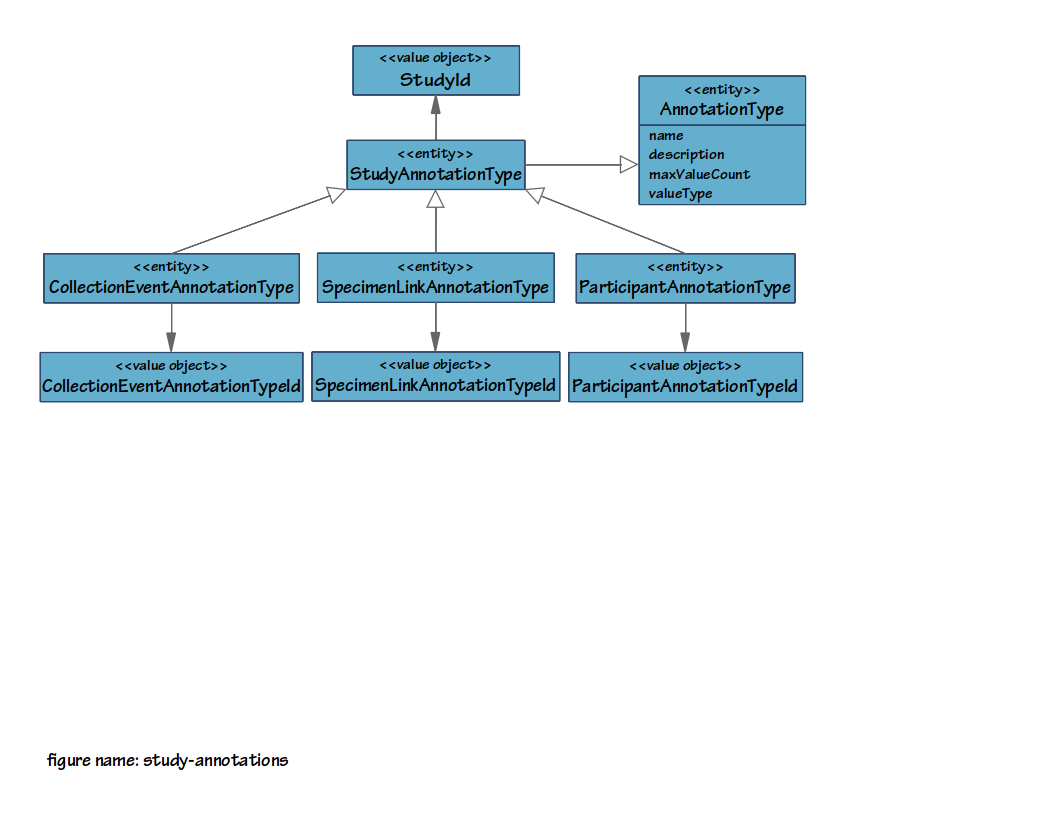
\includegraphics[trim={9mm 108mm 64mm 9mm}, clip,
    width=0.8\textwidth]{images/study-annotations}
  \caption{Study annotation entities}
  \label{fig:study-annotations}
\end{figure}

An annotation type has a short identifying name that is unique to the study. A
description can also be defined but is optional. The \texttt{valueType} can be
one of:

\begin{table}[!htbp]
\renewcommand{\arraystretch}{1.1}
\begin{tabularx}{\textwidth}{@{\hspace{6pt}} >{\ttfamily}l X }

  String & an alphanumeric string.\\
  Number & a number, either integer or decimal.\\
  Date & date string, usually of the form \emph{YYYY-MM-DD HH:MM}.\\
  Select & a value selected from a predefined list.\\

\end{tabularx}
\end{table}

When \texttt{valueType} is assigned to be of type \texttt{Select},
\texttt{maxValueCount} is the number of of items that can be selected from the
predefiend list. If only one value is allowed, then \texttt{maxValueCount} has
a value of 1. If an unlimited number of values are allowed then,
\texttt{maxValueCount} has a value of 0.

\subsection*{CollectionEventTypeAnnotationType}

A \valobjtarget{CollectionEventTypeAnnotationType} is used to to
configure a collection event type to use an annotation. When
\texttt{required} is set to true the annotation value is not allowed to be
empty.

An example of an annotation on a collection even type can be consent given by
the participant at the collection visit.

\subsection*{SpecimenLinkAnnotationType}

A \valobjtarget{SpecimenLinkAnnotationType} is used to to configure a specimen
link type, within a processing type, to use an annotation. When
\texttt{required} is set to true the annotation value is not allowed to be
empty.

An example of an annotation type on a specimen link can be the PMBC count on
the collected specimen.

\subsection*{ParticipantAnnotationType}

A \valobjtarget{ParticipantAnnotationType} is used to to configure a an
annotation for a participant. When \texttt{required} is set to true the
annotation value is not allowed to be empty.

An example of an annotation on a participant can be their gender.

\section {Study Aggregate Commands}

The commands handled by the study aggregate are listed below.

\subsection*{StudyCreateCommand}

Used to create a study. A study can be created at any time. The arguments are:
\texttt{name (String)} and \texttt{description (String)}. The name used to
refer to the study and is usually an acronym. The description describes the
study and is usually the words that make up the acronym.

\subsection*{StudyUpdateCommand}

Used to update a study's name, description, or both. The arguments are:
\texttt{studyId (String)}, \texttt{name (String)} and \texttt{description
  (String)}. The studyId is the study's unique identifier. The name contains
the updated. The description contains the updated description. If either name
or description is not to be updated, it should contain the original value.

\subsection*{StudyEnableCommand}

Used to enable a study. Once enabled the study is ready to collect and process
specimens from participants. The single argument is \texttt{studyId (String)}
is the study's unique identifier.

\subsection*{StudyDisableCommand}

Used to disable a study. A study may be disabled because no more specimen
collection will be done with it, or because it requires configuration
changes. Once disabled the study can no longer collect and / or process
specimens from participants. The single argument is \texttt{studyId (String)}
is the study's unique identifier.

\subsection*{CreateSpecimenGroupCommand}

Used to create a specimen group in a study. The arguments are: \texttt{studyId
  (String)}, \texttt{name (String)}, \texttt{description (String)},
\texttt{anatomicalSourceId (String)}, \texttt{preservationId (String)}, and
\texttt{specimenTypeId (String)}. The studyId is the study's unique
identifier. The name describes the specimen group. The description provides
more details for the speciment group.  The anatomicalSourceId is used to
identify anatomical source on the participants whre this group belongs to.  The
preservationId is used to record how this group is stored.  The specimenTypeId
identifies the type of specimens contained in this group.

\subsection*{DeleteSpecimenGroupCommand}

Used to delete a specimen group from the study. The arguments are:
\texttt{studyId (String)} and \texttt{specimenGroupId (String)}. The studyId is
the unique identifier for the study. The specimenGroupId is the unique
identifier for the specimen group.

